\documentclass[UTF8]{ctexart}
\title{CPU大作业报告}
\usepackage{graphicx}
\usepackage{wrapfig}
\usepackage{fullpage}
\usepackage[margin=0.5in]{geometry}

\begin{document}

\noindent
\large\textbf{CPU大作业报告} \hfill \textbf{苏起冬} \\
\normalsize Computer System(I) 2018 Fall \hfill 517030910415 \\
\today
	
\section{整体架构}
	\begin{wrapfigure}[12]{r}{9.5cm}
	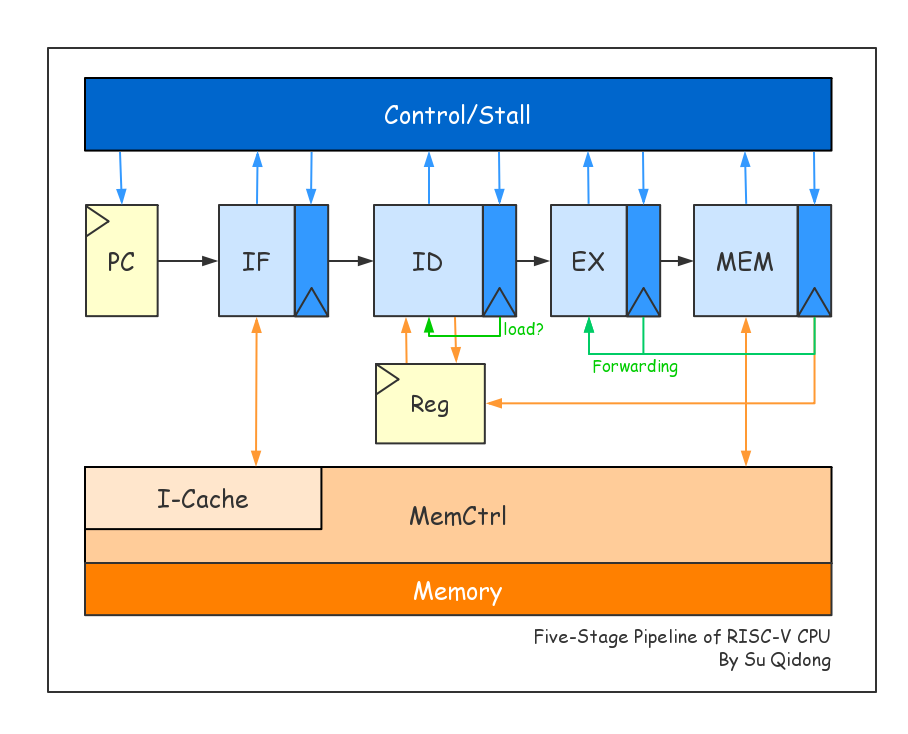
\includegraphics[width=9cm]{arch.png}
	\end{wrapfigure}

	本项目是一个使用Verilog HDL语言实现的能在Basys3上运行RISC-V指令集的一个CPU。最初的设计目标就是不仅要能通过仿真,而且必须可以在真实硬件上面运行,所以整体架构比较简单,主要目标是提高效率和可靠性。CPU可以在100MHz的频率下工作。
	
	整体结构是传统的五级流水架构,如右图所示。
	
	\paragraph{MemCtrl} 是一个状态机,用于处理来自IF和MEM两阶段对于内存的访问需求,并作出仲裁。目前的做法是MEM的请求优先。写入一个字需要5周期,访问板载内存上的一个字需要5周期,通过IO访问的话需要8周期(不计uart通信时间)。
	\paragraph{I-Cache} 一个集成在MemCtrl中的指令缓存,大小为256×4字节。有了I-Cache之后,在命中的情况下可以实现一个时钟周期取指令,大大减少了读取指令的时间,使流水线可以真正工作起来。256条指令基本上能容纳一个函数。
	
	MemCtrl(包括I-Cache)占据下图黄色部分。
	
	\paragraph{IF} 负责读取指令,是一个状态机。在读取完一条指令之后会进行预解码,如果是一条分支语句,则阻塞住流水线的之前阶段,直到这条分支语句计算出下一条语句的地址。(并没有做分支预测)
	
	\begin{wrapfigure}[12]{l}{5.5cm}
		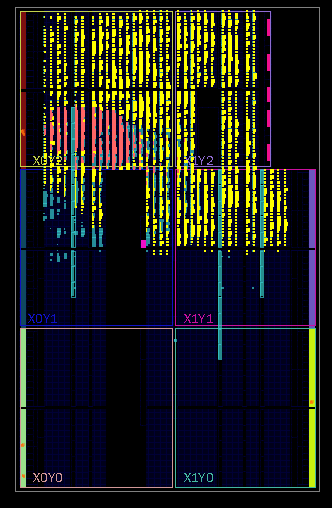
\includegraphics[width=5cm]{impl.png}
	\end{wrapfigure}
	
	\paragraph{ID} 负责解码。这个部分占用的面积(右图红色区域)比较大,看起来还有很多改进的空间。解码之后如果发现下一条指令是load指令并且与当前指令有依赖关系,则在当前指令后面插入一条空指令。
	

	
	\paragraph{EX} 负责执行。
	\paragraph{MEM} 负责进行内存操作,是一个状态机。如果目前处理的指令有内存操作,则阻塞流水线的之前阶段,直到MemCtrl返回done信号。
	\paragraph{控制模块} 控制模块主要做两件事情:控制stall和修改pc值。这是一个简单的组合逻辑,接收各个部件对于流水线stall的请求,计算后广播给各个部件。
	\paragraph{*D-Cache} 我在memctrl里面做了一个简易的数据缓存,但是很难符合时序要求,很难在一个周期的时间里取到数。而且经过试验发现对于性能的改进并不是那么明显,占用面积又非常大,所以没有启用。但是可以通过宏定义在memctrl中启用dcache的功能。(功能上还不完善)
	
\section{遇到的问题}

	\subsection{时序设计}
		\paragraph{误区} 我一开始以为在一个周期内做的事情越多越好,但是后来发现完全不是这么一回事。组合逻辑一复杂,逻辑门的延时就会变大,就容易无法满足时序要求,无法升高频率。设计的时候应该注意流水线的各个阶段之间所用的时间应该尽量均匀。
		
		\begin{wrapfigure}[13]{l}{8.5cm}
		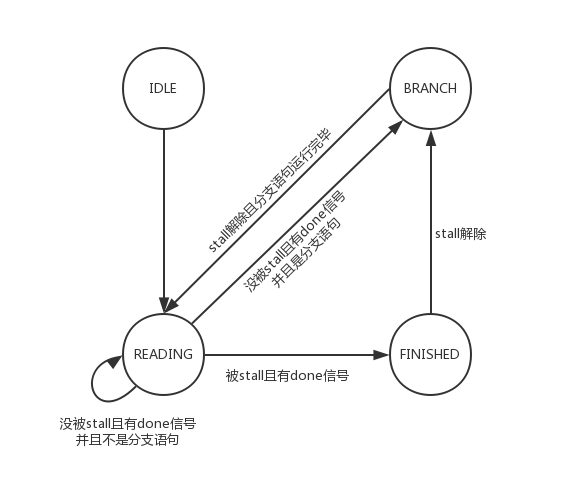
\includegraphics[width=8cm]{IF_stage.png}		
		\end{wrapfigure}
		
		\paragraph{不同模块之间的配合} IF、MEM、MemCtrl、PC等模块之间的时序关系比较复杂,如果要充分利用起每一个周期,需要仔细考虑它们之间的关系。我选择使用状态机来实现各个模块。左图是IF的状态转移图。
		
		IF在取完一条指令之后(此时memctrl的busy为0,done为1)会立即请求下一条语句,也就是说这个busy为0的状态只会维持一个周期。而MEM阶段在完成一次读写操作之后(此时memctrl的busy为0,done为1)这个周期是被空出来的,否则流水线仍然会被阻塞住(因为只要MEM有请求,流水线就会被阻塞住)。在这个空出来的周期里,可以完成pc的修改,IF也可以抢先发起请求。
		
		IF发起请求之后,MemCtrl会读完这条指令(无论这个过程中MEM阶段是否遇到读取指令)。在这个过程中,MEM阶段遇到了读取指令,那么流水线一直处于stall状态。如果此时IF请求的指令读完了,并且当前流水线被stall住了,那IF就将读到的指令暂存起来,直到stall解除再恢复流水线的运行。
		

		
		\paragraph{期待改进} 现在这个CPU的设计应该说是非常简单,但是时钟频率最高也只能到达110MHz左右,无法继续升高频率,这和预想中的效率还有一些差距。
	\subsection{综合、实现}
		\paragraph{底层=黑箱} 对于综合机制了解的不多。Vivado中有许多Systhesis、Implementation的策略可供选择,但是我对它们并没有什么了解,也不知道修改那些参数会有什么后果,基本就是胡乱选择。现在产生的bitstream文件基本是在Flow\_PerOptimized\_high和Performance\_ExtraTimingOpt策略下完成的。
	\subsection{调试}
		\paragraph{模拟和实际的区别} 在模拟阶段发现代码有错误还是很容易改正的。最可怕的是可以过模拟,但是烧到FPGA上之后运行不正常。因为硬件上的调试手段并不多。在这种情况下,我选择使用vivado自带的调试核,在设定了一定的触发条件之后,它可以记录一段时间内信号的变化。对于调试来说非常实用。
		
	\begin{thebibliography}{9}
		\bibitem{lsl}
		雷思磊.
		\emph{自己动手写CPU},
		电子工业出版社, 2014.
		\bibitem{hzb}
		胡振波
		\emph{教你设计CPU——RISC-V处理器}
		人民邮电出版社,2018.
	\end{thebibliography}
	
\end{document}
